\documentclass[12pt]{article}
\usepackage{graphicx}
%\documentclass[journal,12pt,twocolumn]{IEEEtran}
\usepackage[none]{hyphenat}
\usepackage{gensymb}
\usepackage{commath}
\usepackage{listings}
\usepackage[english]{babel}
\usepackage{caption}
\usepackage{amssymb}
\usepackage{hyperref}
\usepackage{enumitem}
\usepackage{booktabs}
\usepackage{array}
\usepackage{amsmath}   % for having text in math mode
\usepackage{listings}
\lstset{
  frame=single,
  breaklines=true
}
%New macro definitions
\newcommand{\mydet}[1]{\ensuremath{\begin{vmatrix}#1\end{vmatrix}}}
\providecommand{\brak}[1]{\ensuremath{\left(#1\right)}}
\providecommand{\norm}[1]{\left\lVert#1\right\rVert}
\newcommand{\solution}{\noindent \textbf{Solution: }}
\newcommand{\myvec}[1]{\ensuremath{\begin{pmatrix}#1\end{pmatrix}}}
\let\vec\mathbf


\begin{document}
\begin{center}
\textbf\large{CLASS-9\\CHAPTER-10 \\ CIRCLES}
\end{center}
write \textbf{True} or \textbf{False} and justify your answer in each of the following:
\begin{enumerate}
\item Two chords $AB$ and $CD$ of a circle are each at distances $4 cm$ from the centre The $AB=CD$.
\item Two chords $AB$ and $AC$ of a circle with centre $O$ are an the opposite sides of $OA$ Then $\angle 0AB = \angle 0AC$
\item Two congruent circles with centres 0 and 0 intersect at two points $A$ and $B$ Then $\angle AOB= \angle AOB$
\item Through three collinear points a circle can be drawn
\item A circle of radius $3 cm$ can be drawn through two points $A,B$ such that $AB= 6cm$
\item If AOB is a diameter of a circle and $C$ is a point on the circle, then $AC^2+B^2=AB^2.$
\item $ABCD$ is a cyclic quadrilateral such that $\angle A=90\degree ,\angle B=70\degree, \angle C=95\degree \text{ and }\angle D=105\degree$
\item If A,B,C,D are four points such that $\angle BAC=30\degree, \angle BDC=60\degree$, then D is the centre of the circle through A,B  and C.
\item If A,B,C and D are four points such that $\angle BAC =45\degree \text{ and }\angle BDC=45\degree$, then A,B,C,D are concyclic.
\item ln Fig -10.10 if AOB is a diameter and $\angle ADC=120\degree \text{ then }\angle CAB=30\degree$
\begin{figure}[h!]
 \begin{center} 
	 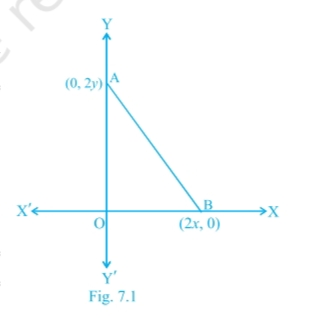
\includegraphics[width=\columnwidth]{image.jpg}
 \end{center}
\caption{}
	\label{}
\end{figure}
\end{enumerate}
\end{document}
